\chapter{Experimental Setup}
Every theory needs to have experimental proof to show it's compatibility. Particle physics is tested on
the colliders.
% \\
% Before the Large Hadron Collider era the Standard Model was experimentaly tested up to the scale of ~TeV.
% But there was a strong demand to raise the scale and implement the studies of electroweak symmetry breaking
% and Higgs mechanism.
% Physics beyond SM is also of interest on the scales above 1 TeV.
% The Large Hadron Collider\cite{LHCmachine} was providing the collisions with a centre-of-mass energy
% up to 8 TeV which is an eightfold increase of the scale compared to the previosly most powerful collider TEVATRON.
% \\


This chapter is devided into three parts.
The first part is denoted to the description of the Large Hadron Collider. The second part of the 
chapter is revealing the CMS detector construction and features in more detail as it was used to produce the final
results of this work. The third and the last part of this chapter is about the upgrade plans for the
CMS detector to operate with higher energies and luminosities.

%%%%%%%%%%%%%%%%%%%%%%%%%%%%%%%%%%%%%%
%%%%%%%%%%%%%%%%%%%%%%%%%%%%%%%%%%%%%%
%%%%%%%%%%%%%%%%%%%%%%%%%%%%%%%%%%%%%%
\section{Large Hadron Collider}\label{sec:LHC}

The fastest protons in the world, ever controlled by human, are alive in Switzerland at CERN.
The Machine which can manage the operation of these protons is called Large Hadron Collider(LHC). 
The LHC is a ring-shape tunnel 26.7 km long  placed 45 - 170 m underground. 
Inside the tunnel there are two rings with vacuum tubes where proton(or lead nuclei) beams are circulating in different directions.
There are four locations where the rings are crossing and the protons can collide with each other. 
The designed center-of-mass energy for those collisions is $\sqrt{s}$ = 14 TeV, which means 7 TeV in one direction.


Not to get out of the ring 7 TeV protons are guided by 8 T superconducting magnets. 
For optimal usage of these magnets one needs to preaccelerate and preform the proton bunches.
For this purpose LHC is supported by preacceleration system.


The way of the protons literally starts from a bottle of hydrogen gas.
H2 molecules are entering metallic cylinder (duoplasmatron[?]) with electron gas under magnetic field  where they are smashed 
into atoms and stripped off the electrons. The protons produced by a duoplasmatron have to satisfy very stringent needs of the LHC -- 
many high intensity proton bunches (2808 per LHC ring) with small transverse and well defined longitudinal emittances.
To reach the stated goals the following acceleration injector chain is used(Fig. \ref{fig:AccelCERN}): 

\begin{figure}[t]
  \centering
  %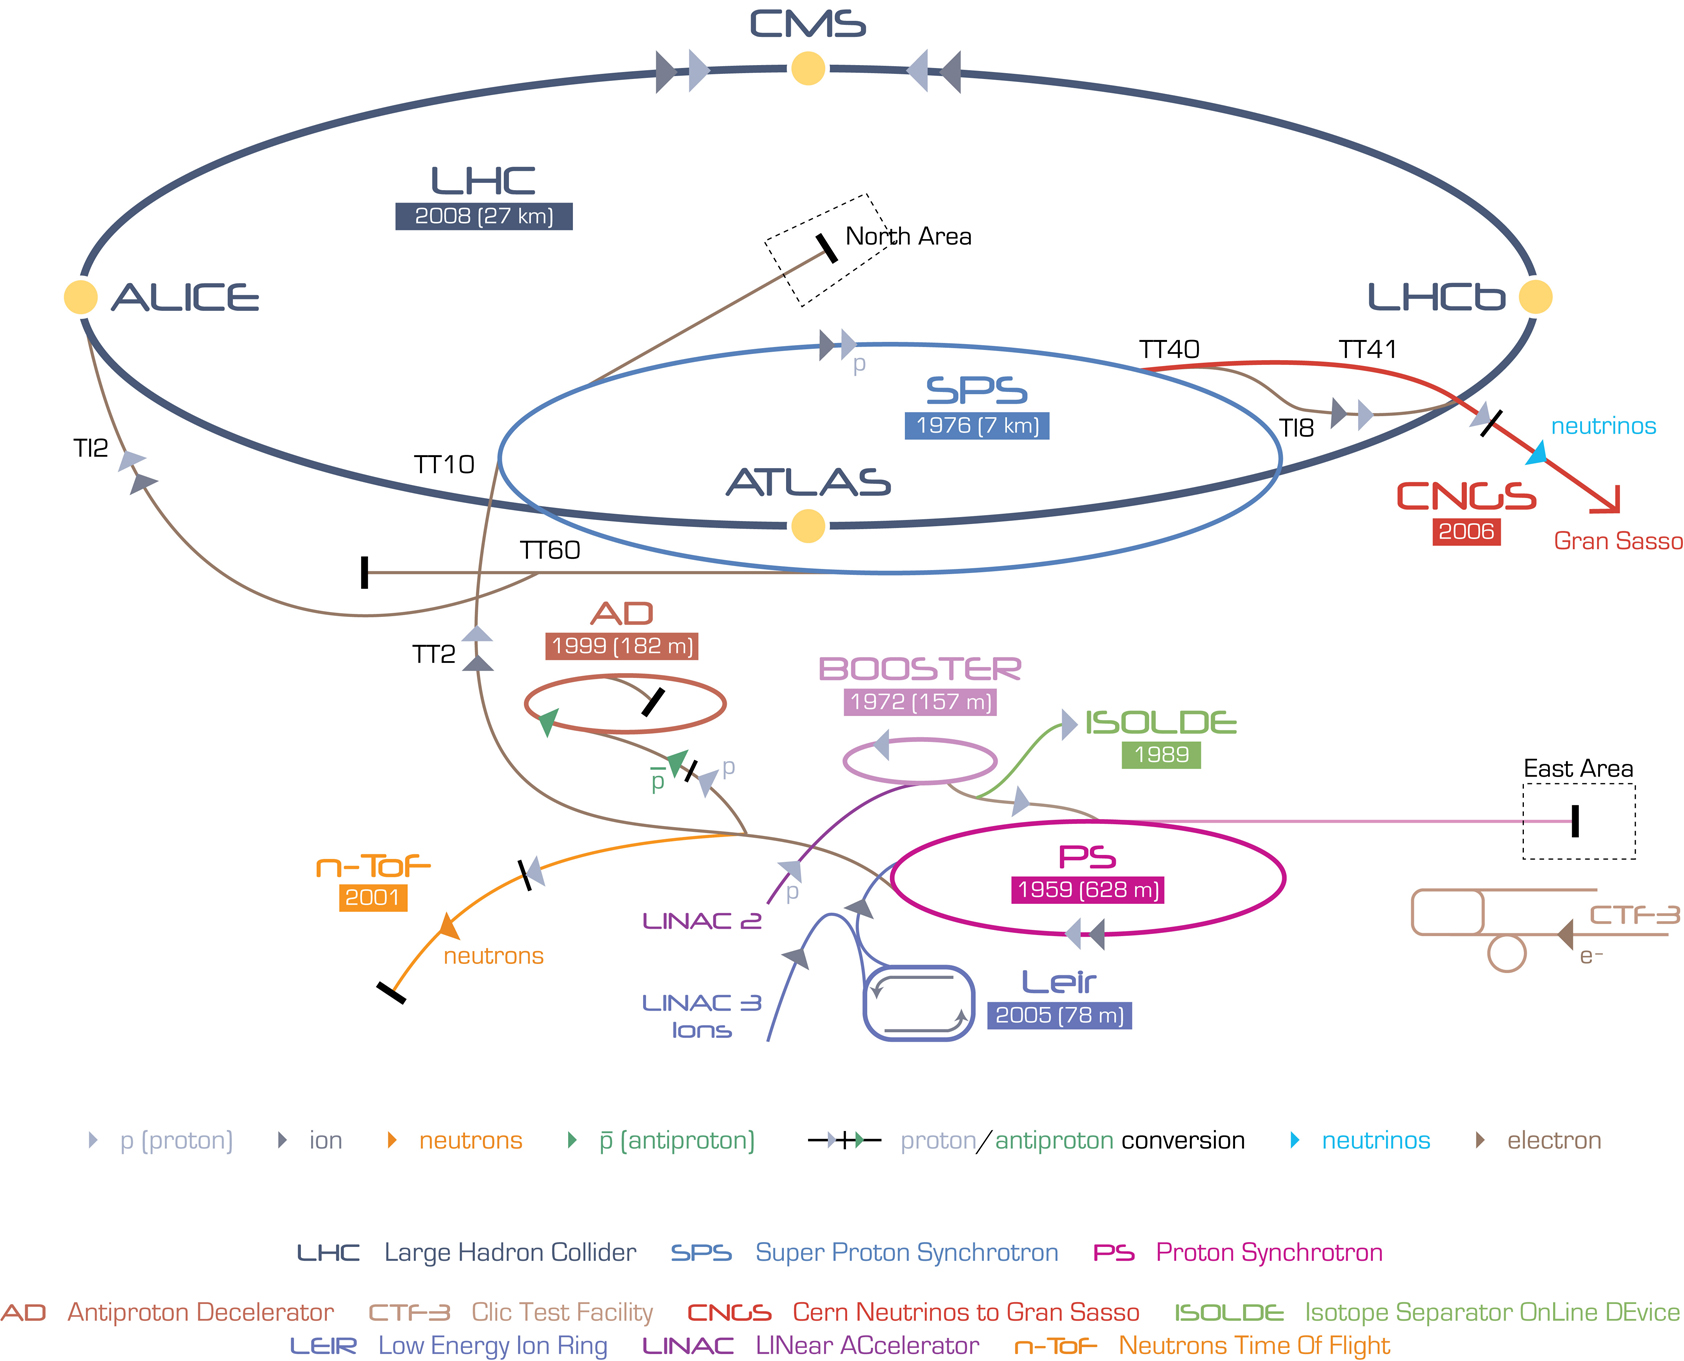
\includegraphics[width=0.6\textwidth]{02_experimental_setup/plots/Cern-Accelerator-Complex.png}
  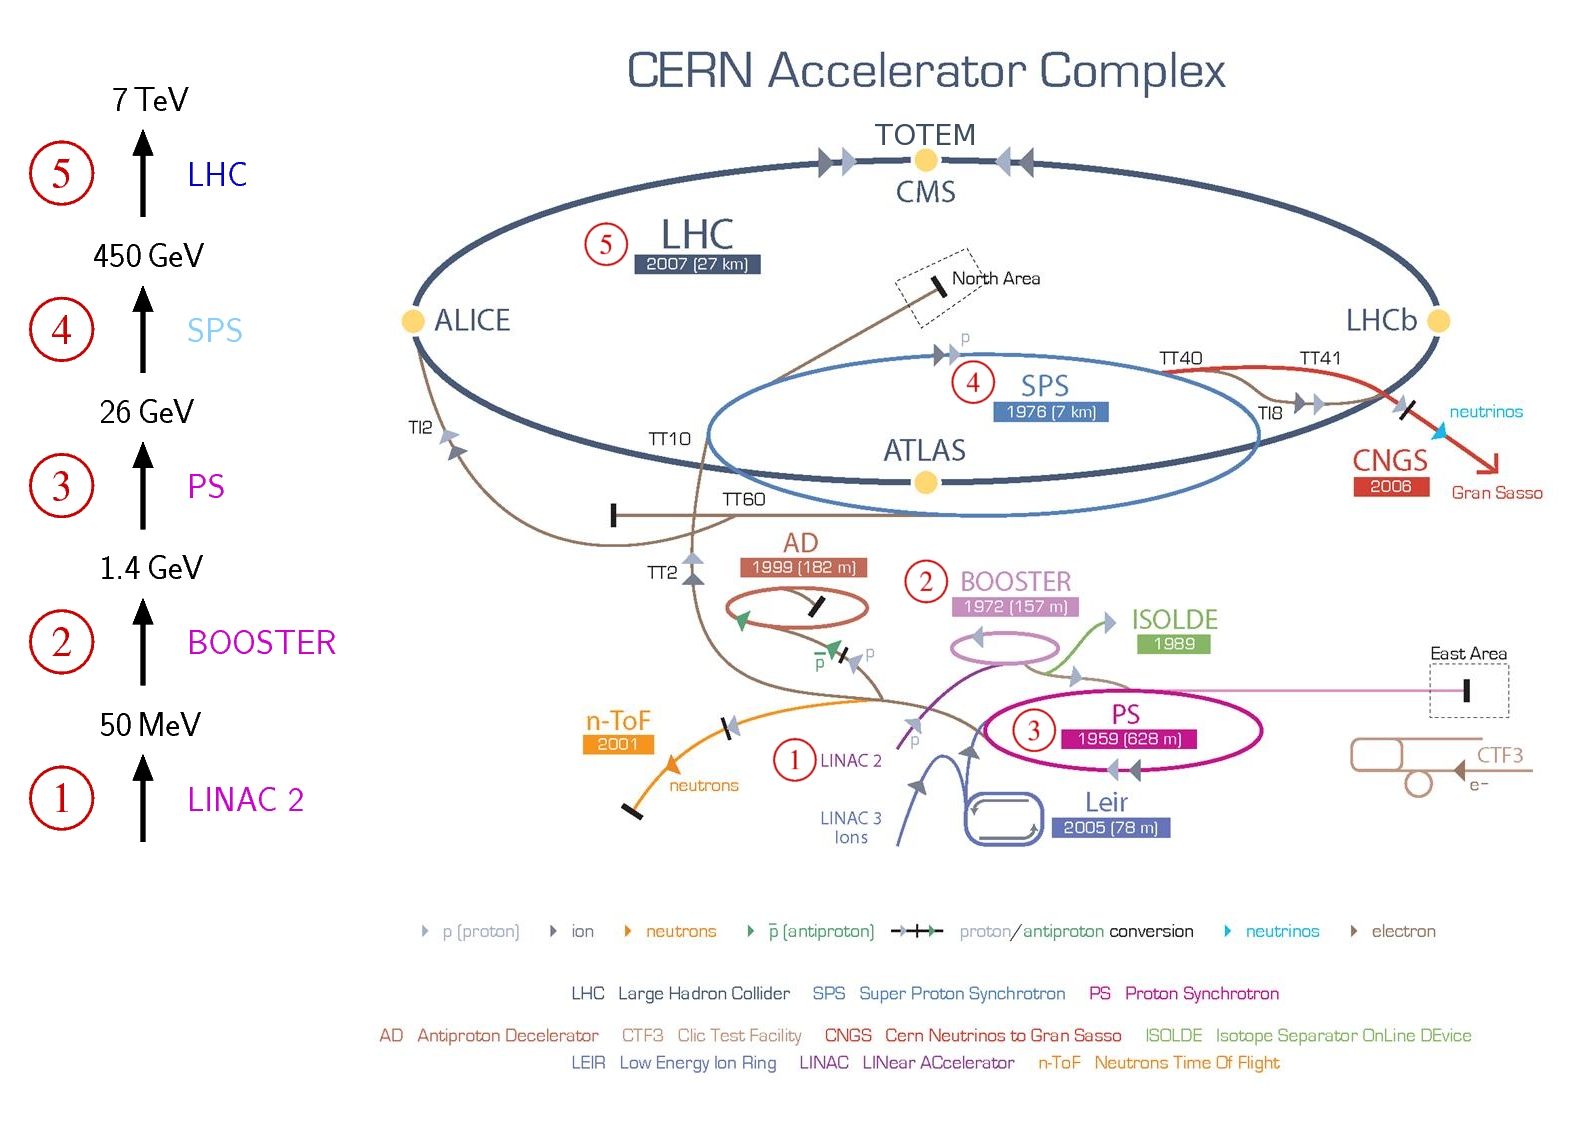
\includegraphics[width=0.8\textwidth]{02_experimental_setup/plots/Cern-Accelerator-Complex-2.png}
  \caption{The complex of accelerators at CERN with their length and particles being accelerated inside.}
  \label{fig:AccelCERN}
\end{figure}

\begin{itemize}
 \item[--] Protons first enter the \textit{Linac2}[?] where they are accelerated up to 50 MeV and sent to Proton Synchrotron Booster (PSB);
 \item[--] \textit{PSB}[?] is composed of four synchrotron rings (to avoid charge repulsion) which raise the energy of the particles to 1.4 GeV
 for injection into the Proton Synchrotron (PS);
 \item[--] \textit{PS}[?] increases the energy up to 26 GeV and takes 3.6 s to get injection to the Super Proton Synchrotron (SPS); 
 \item[--] \textit{SPS}[?] is the second largest accelerator at CERN which comes out with 450 GeV protons injected to LHC.
\end{itemize}

The important accelerator characteristic to perform experimental measurement is the number of coinciding protons 
in coincidence area per time called \textit{instantaneous luminosity} $\mathcal{L}$. The designed value 
at the LHC is $\mathcal{L} = 10^{34}$ cm$^{-2}$ s$^{-1}$. The accelerator was providing $\mathcal{L} = 7.7 \cdot 10^{33}$ cm$^{-2}$ s$^{-1}$
during the run in 2012.

Integral of instantaneous luminosity over the time
is defined as \textit{integrated luminosity} $L$: 
\begin{equation}\label{eq:lumi}
  L  = \int\mathcal{L}dt.
\end{equation}
LHC provided 23.3 fb$^{-1}$ of integrated luminosity for the run in 2012 from which 21.8 fb$^{-1}$ were
recorded by the Compact Muon Solinoid (CMS) detector which is seen from the Fig.\ref{fig:LumiCMS}

\begin{figure}[t]
  \centering
  %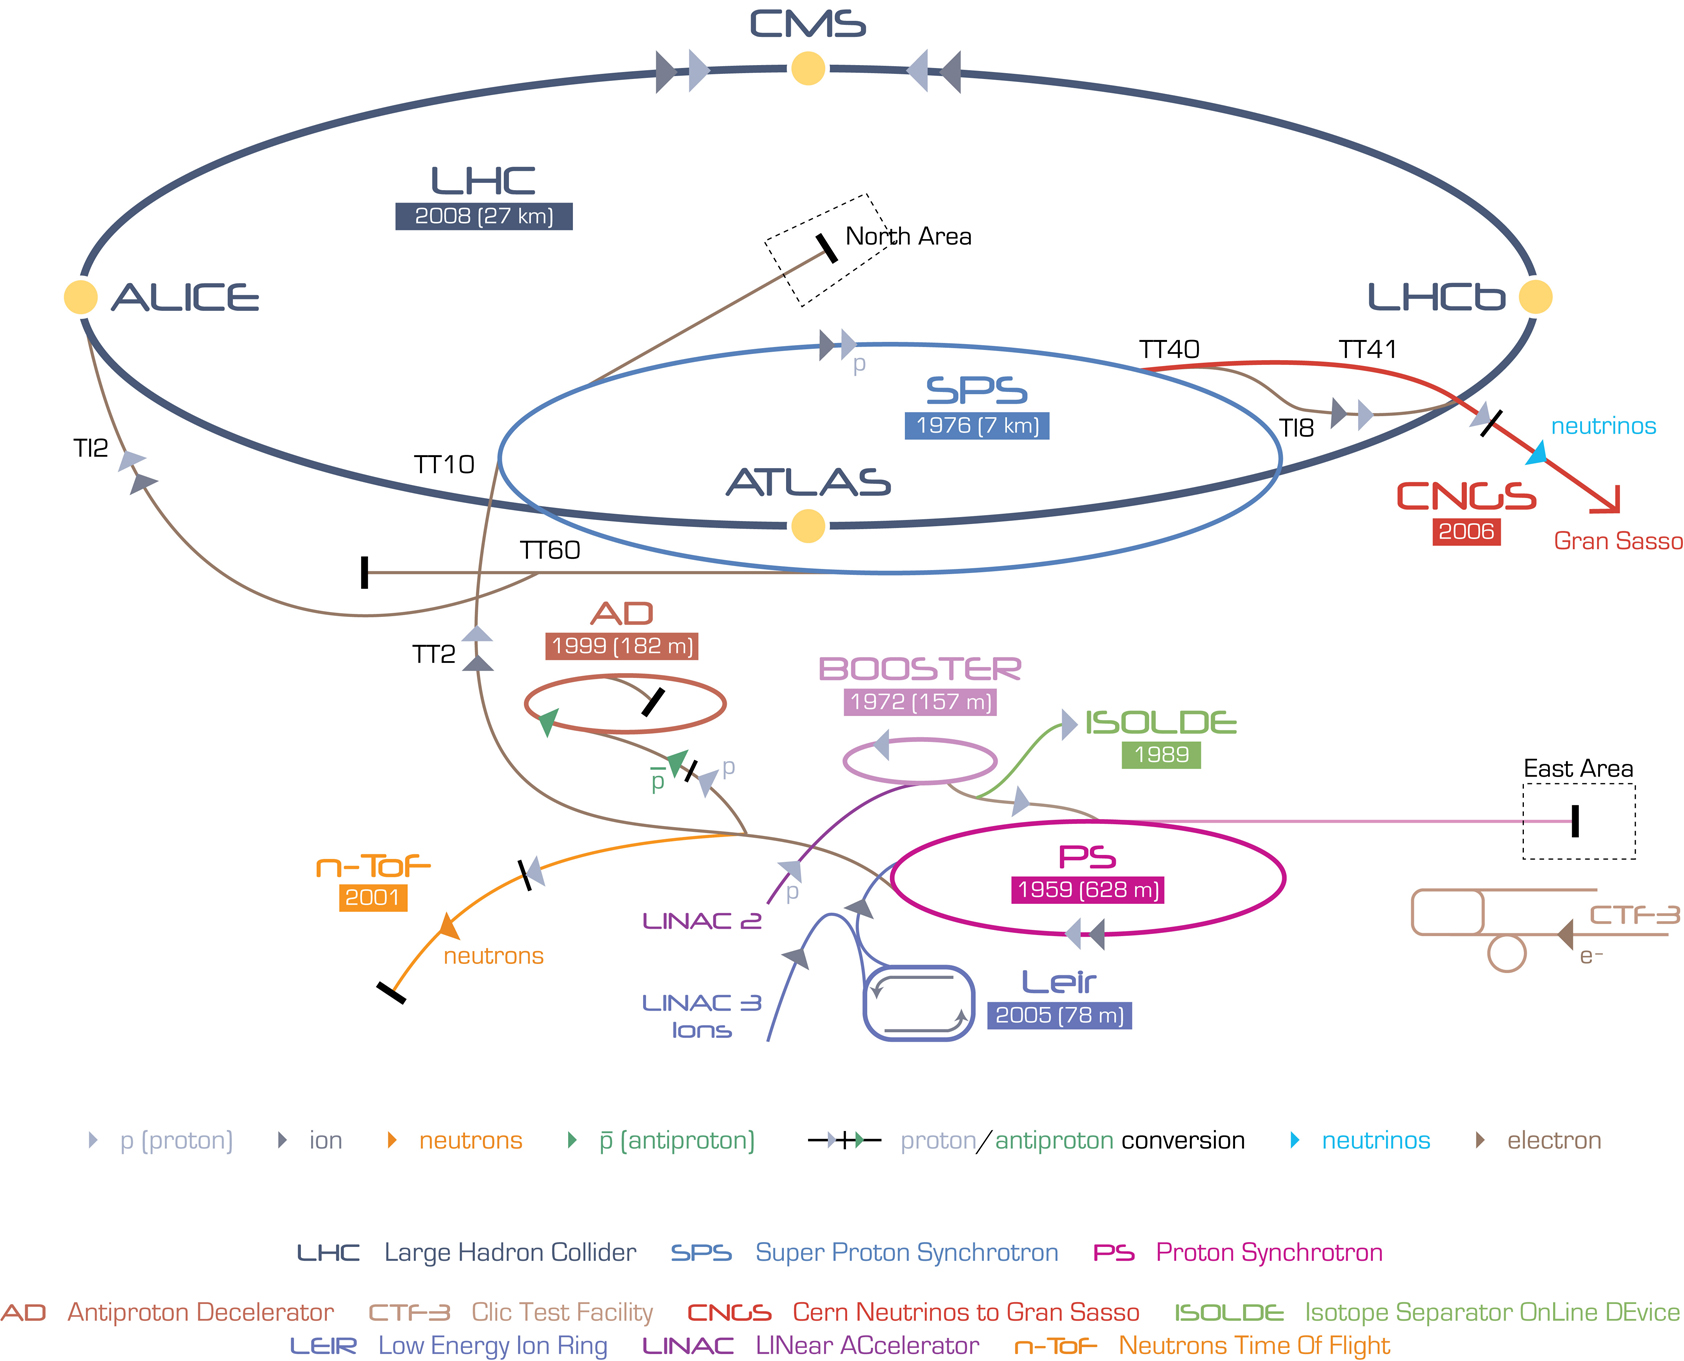
\includegraphics[width=0.6\textwidth]{02_experimental_setup/plots/Cern-Accelerator-Complex.png}
  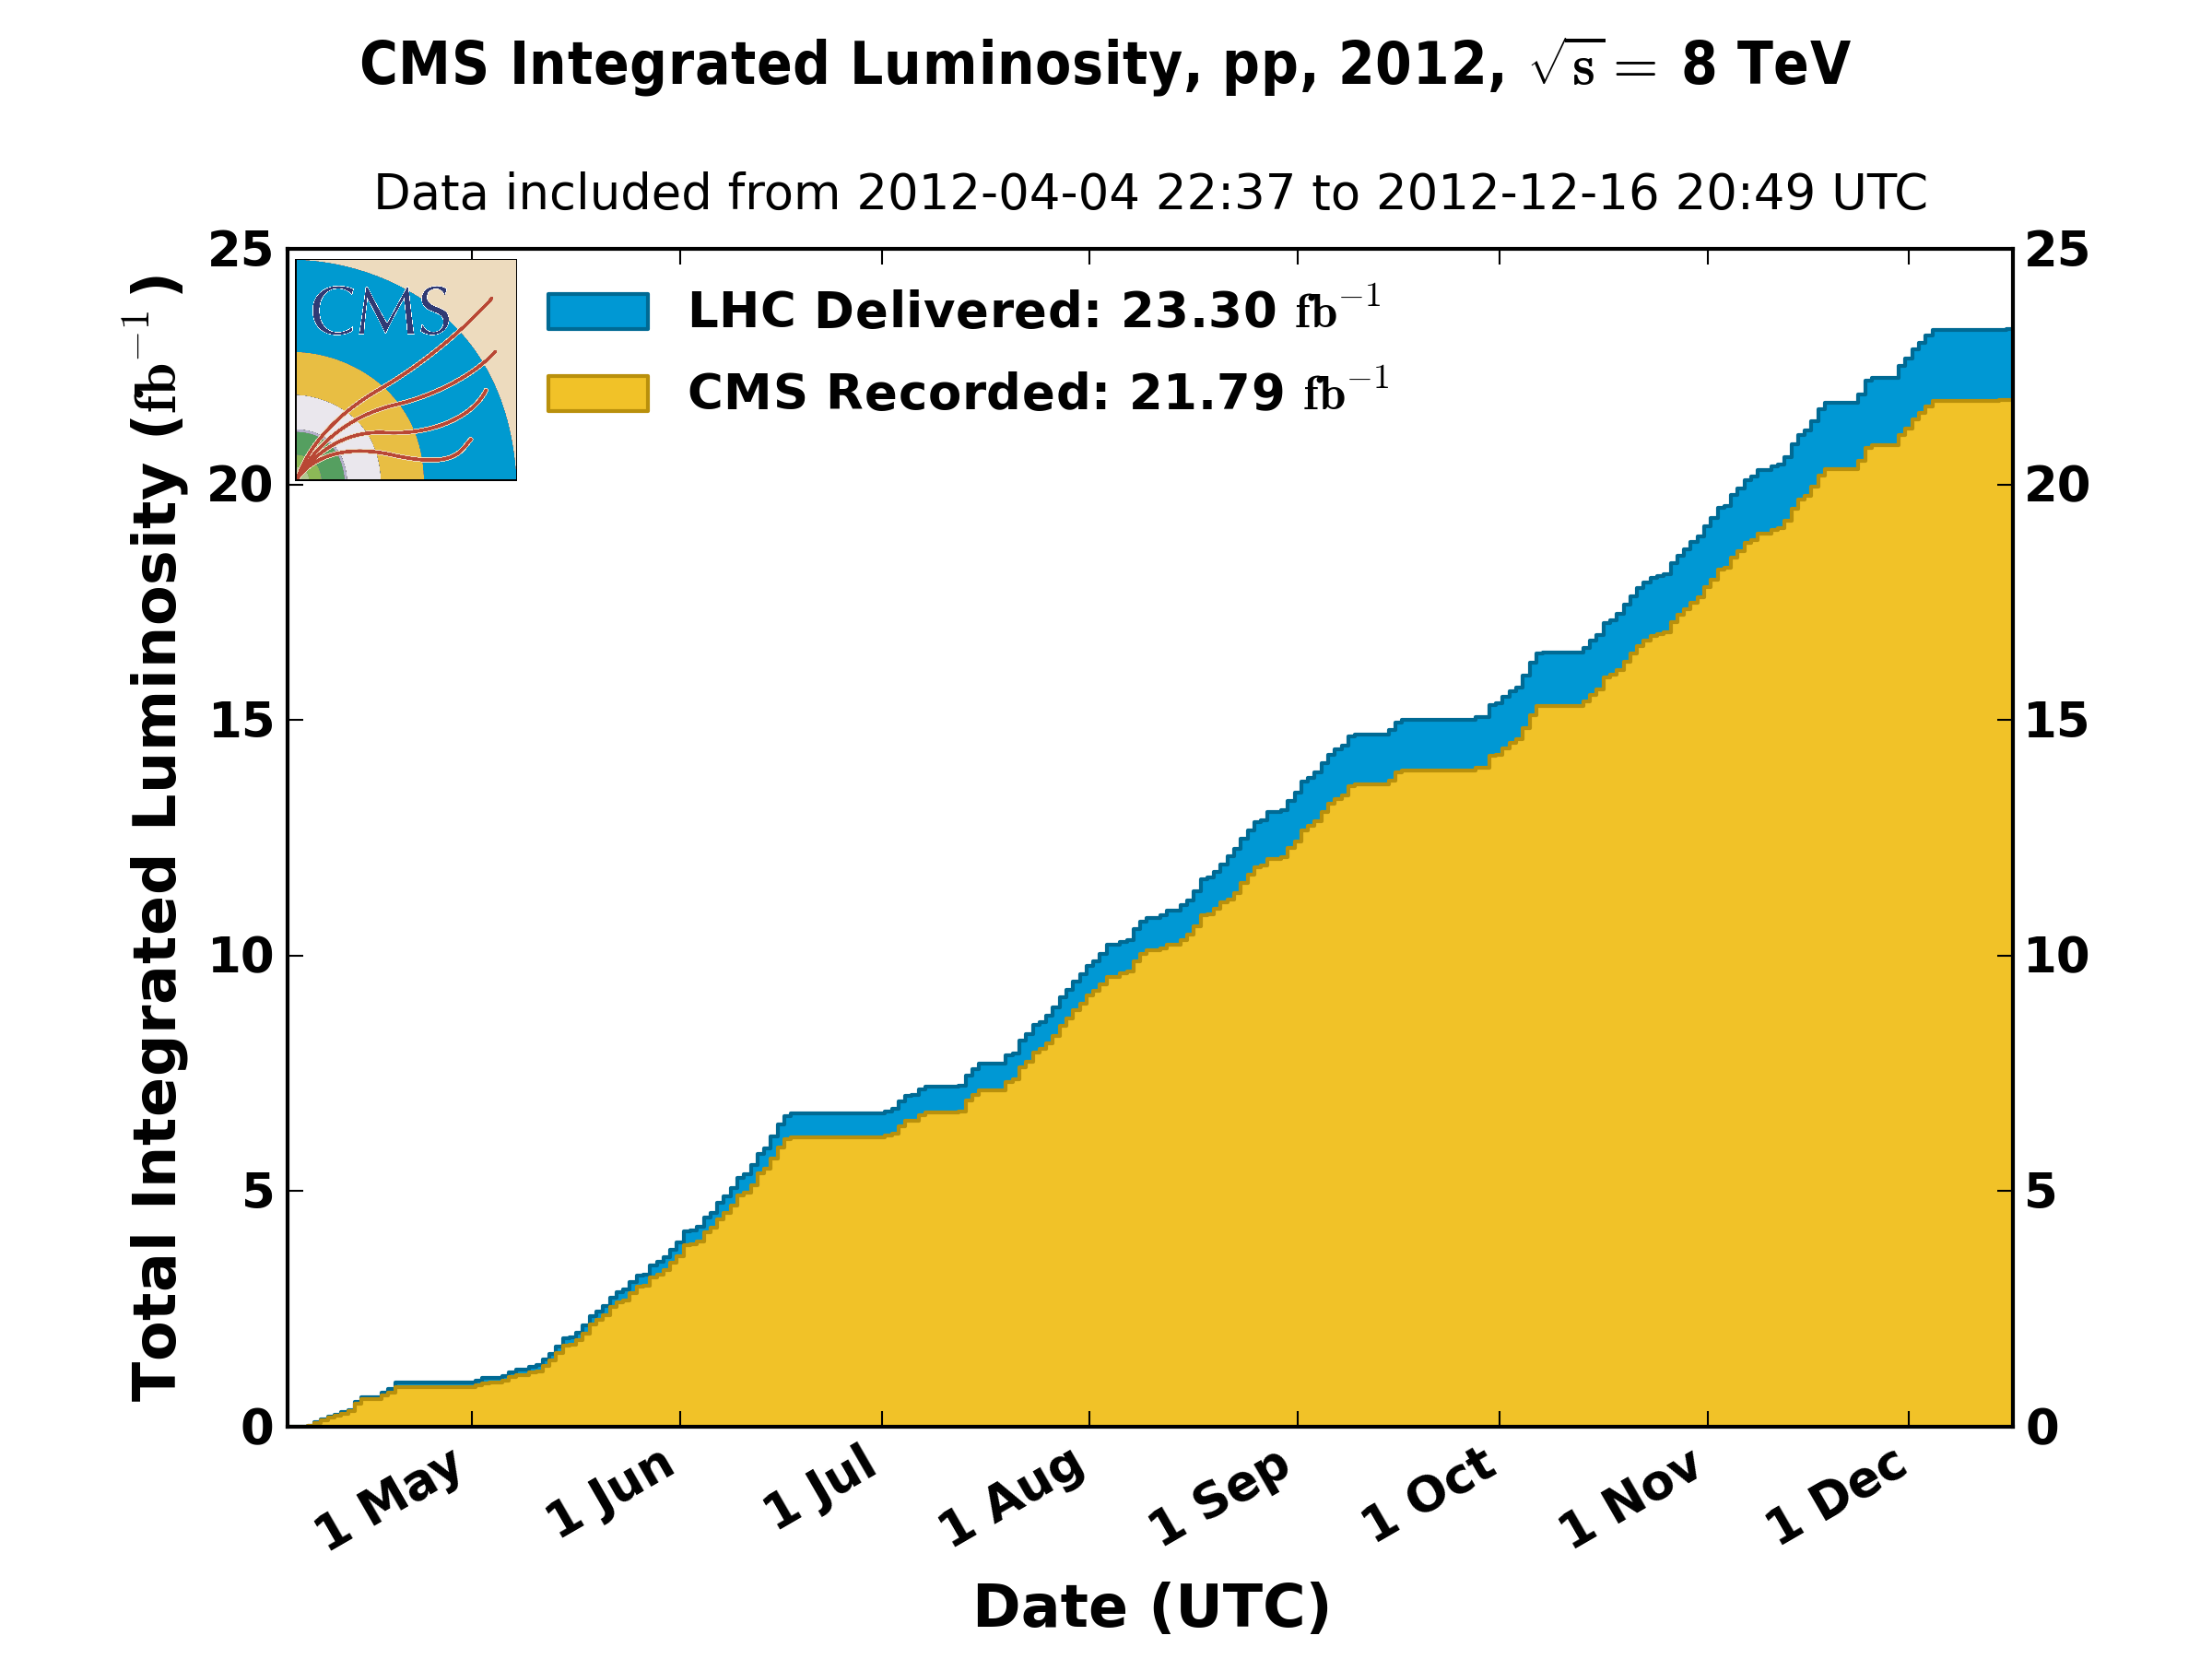
\includegraphics[width=0.6\textwidth]{02_experimental_setup/plots/int_lumi_per_day_cumulative_pp_2012.png}
  \caption{Cumulative luminosity versus day delivered (blue) and recorded by the CMS (orange) for proton-
  proton collisions during stable beam time in 2012.}
  \label{fig:LumiCMS}
\end{figure}

During the 2012 LHC run period $3.16 \cdot 10^16$[?] protons were delivered which means only ~$1$ mm$^3$ of Hydrogen gas 
under the normal conditions is needed (taken the efficiency of proton source to account[?]). 
%http://www.lhc-closer.es/1/3/10/0
%https://indico.cern.ch/event/219327/ -- slide 11

The measurements of collision products are done with the complex particle detectors. There are four of them, 
\textit{ALICE}, \textit{LHCb}, \textit{ATLAS} and \textit{CMS}, on the LHC
ring, each located around the point where beams of particles of different directions are brought together.
These detectors have different construction thus having slightly different goals.

\begin{itemize}
 \item The ALICE (A Large Ion Collider Experiment)\cite{ALICEtdr} is designed to
 work with the heavy ion collisions. The goal of the ALICE experiment studies is
 the strongly interacting matter in extremely high density state called \textit{quark-gluon plasma}. This 
 state of matter provides a unique possibility to find a bare quark without a pair and also to study the early
 Universe which was so dense at the first moments after the Big Bang.
 \\
 The ALICE detector weights 10000 tonnes and is 26 m long, 16 m high and 16 m wide. It sits on the depth of
 56 m below the ground on the territory of France.
 
 \item The LHCb (Large Hadron Collider beauty)\cite{LHCb} is investigating the $CP$ violation and heavy flavour physics via
 the rare $B$ hadron decays. As the $b\bar{b}$ pairs are mostly produced in the forward and backward directions, 
 and their production cross section is very high there was no need to construct a big and expensive $4\pi$ detector 
 complex. For this reason the LHCb is a one side spectrometer corresponding to the forward beam direction.
 For a better detection of the $b$-decays the LHCb features a movable tracking system which can go very close
 to the beam pipe.
 \\
 The LHCb detector weights 5600 tonnes and is 21 m long, 10 m high and 13 m wide. It sits on the depth of 100 m 
 below the ground on the territory of France.
 
 \item The ATLAS (A Toroidal LHC ApparatuS)\cite{ATLAS} is one of the two general purpose detectors on the LHC. It has many physical
 goals -- from Standard Model examination and Higgs searches to the studies of dark matter, extra dimensions and new physics.
 These tasks are mainly similar to the ones from the CMS experiment (the second general purpose detector on the LHC ring), but
 it uses different technical solutions.
 \\
 The ATLAS machine is built around the beam pipe such that the collision point is located in its center. It consists of the 
 inner tracking system and calorimeter, both surrounded by the barrel (2 T) and toroid magnets (0.5 to 1 T). The muon spectrometer
 is located on the outer layers of the detector.
 \\
 Having a length of 45 m, a height of 25 m and a width of 25 m ATLAS is a largest particle detector complex in the world. While the mass 
 of it is rather low reaching 7000 tonnes. It sits in a cavern 100 m under the ground on the territory of Switzerland.
 
 \item The CMS (Compact Muon Solenoid) is the second general purpose detector on the LHC. A more detailed description of this apparatus will follow in the
 section \ref{sec:CMS}.
 
\end{itemize}


Two much smaller experiments are also located at the LHC ring alongside the four larger ones mentioned above. They are focused on forward particles
researches which do not collide but rather brush past each other and continue their flow along the beam direction. Thus these facilities do not
need to be based around the beam coincidence points. The names of the two experiments are \textit{LHCf} and \textit{TOTEM}.

%%%%%%%%%%%%%%%%%%%%%%%%%%%%%%%%%%%%%%
%%%%%%%%%%%%%%%%%%%%%%%%%%%%%%%%%%%%%%
%%%%%%%%%%%%%%%%%%%%%%%%%%%%%%%%%%%%%%
\section{The Compact Muon Solenoid}\label{sec:CMS}

The analysis presented in this work was performed on the data recorded by the Compact Muon Solenoid (CMS) detector\cite{CMSatLHC} during the 2012
run period in proton-proton collisions with center-of-mass energy $\sqrt{s} = $8 TeV. This section will describe in more detail 
the construction and performance of the CMS machine.

Any particle detector is being constructed with respect to the measurements which are planned to be done on it. Different physical
tasks provide special requirements for specific experimental setup parts. If the plan is to measure Standard Model decays
($W$, $H$, $Z'$ decays with leptons in final state), the detector complex has to comprise a precise electromagnetic calorimetry and 
muon systems for a better lepton reconstruction. To measure the QCD processes with jets in final states, a
good hadronic calorimetry has to provide absolute energy determination with fine resolution. To look for heavy resonances one needs a
precise detection in the central region, perpendicular to the beam direction. Unlike for the low mass particles, where the tracking
has to cover the forward regions. The parts of the detector located in the direction of beam flow are also important to measure the 
total transverse missing energy. A particle identification precision relies much on a magnet system which bands the charged 
particles differently corresponding to their momentum to mass relation and charge. Thus it is important to choose the optimal magnet
shape and power. To gain precise $b$- and $\tau$ identification, silicon
pixel of at least micron resolution and strip detectors have to be operated. 

Taken into account the designed luminosities (see Sec.\ref{sec:LHC}) at the LHC,
the detectors have to deal with multiple interactions per collision - pile up. Not to get distorted by a large amount of particles 
flowing to one sensor unit, the detector must have a fine enough granularity. The designed and bunch spacing of 25 ns 
requires a fast enough readout. Radiation hardness of the materials is very important concidering high luminosity and small
bunch spacing. And in the end the price and feasibility play a crucial role in the detector complex creation.

The CMS facility being a general purpose detector was designed to make it's parts fulfill as many physical goals as possible.
Final onion-like construction of the machine is shown on the Fig. \ref{fig:CMSview}. The overall detector size reaches 28.7 m in length
and 15.0 m in width. The total weight of the facility is 14000 tones, which makes the CMS the heaviest particle detector on the
LHC. Detector is cylindrically symmetric around the beam pipe and also symmetric to left and right sight along the beam direction
relative to the collision point.

\begin{figure}[t]
  \centering
  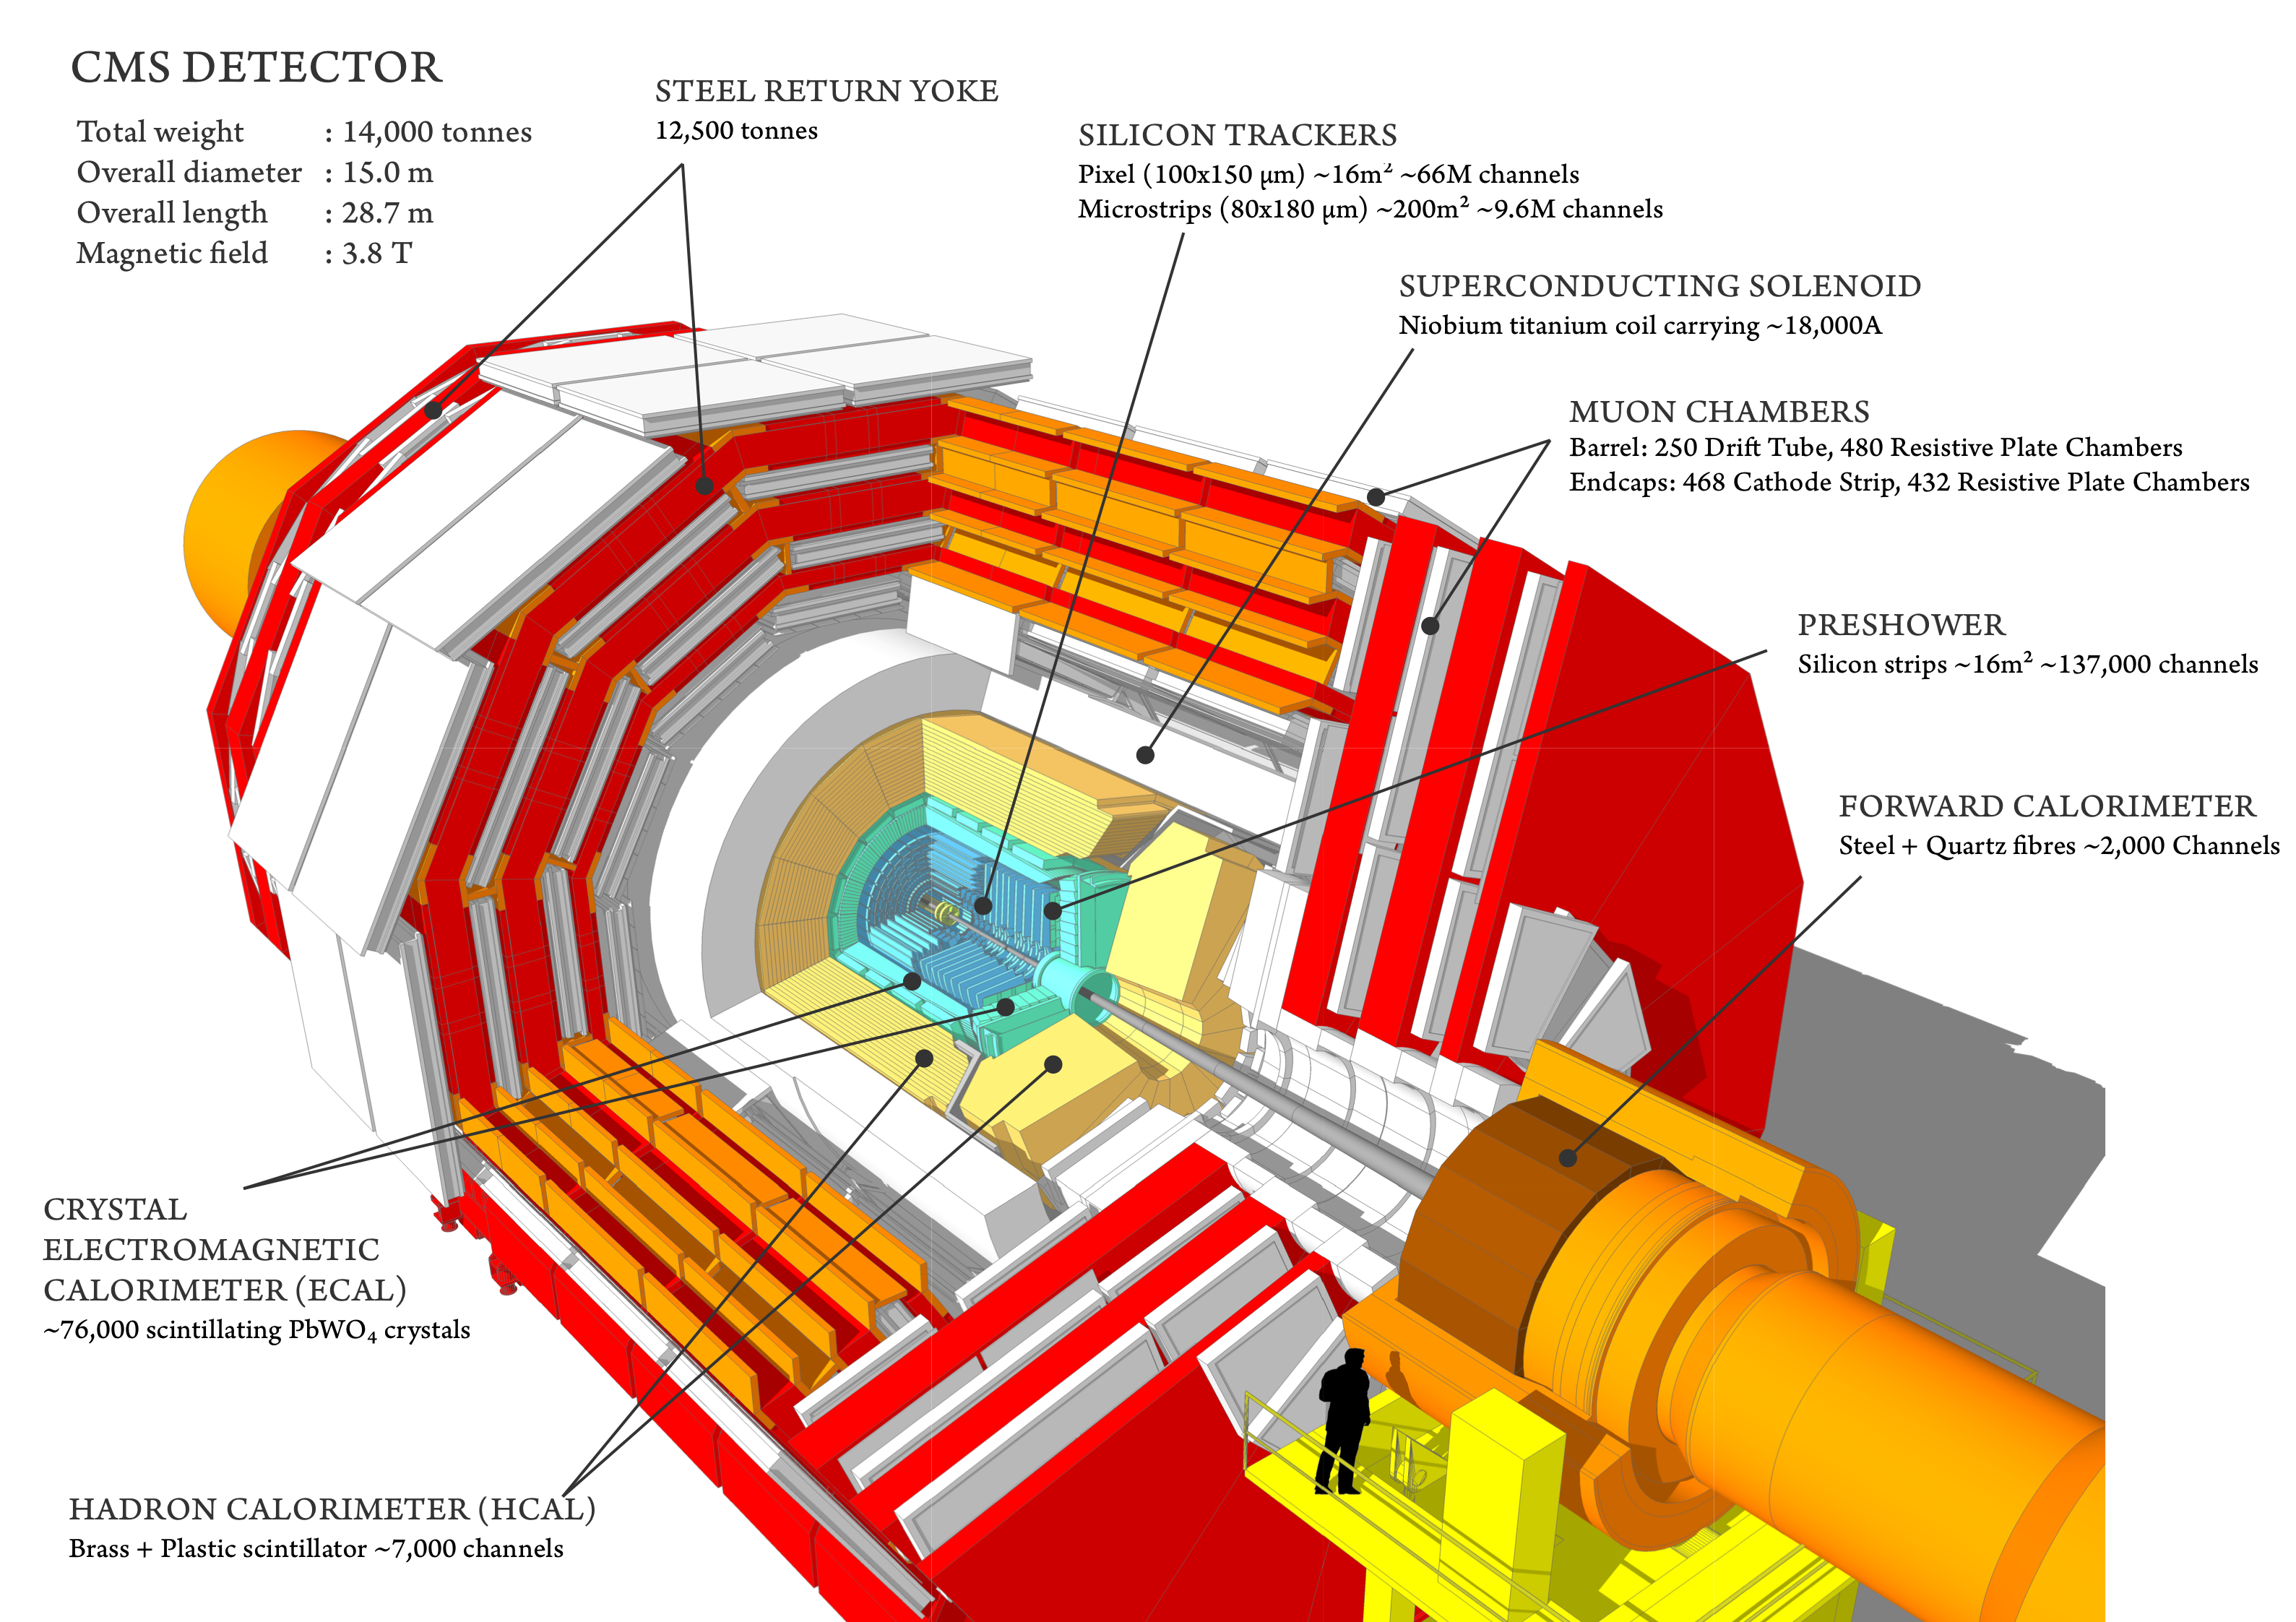
\includegraphics[width=0.8\textwidth]{02_experimental_setup/plots/cms_120918_03.png}
  \caption{Sectional view of the CMS detector with highlighting different components. 
  The LHC beams collide in the center of the machine. The central axis of the detector 
  corresponds to the beam line.}
  \label{fig:CMSview}
\end{figure}

The common coordinate system is important for measurement consistency. For the CMS experiment the origin  
is assumed to be located at the nominal collision point, the $x$-axis is pointing to the center of the 
LHC ring and the $y$-axis is pointing vertically upwards. Thus the $z$-axis points along the beam axis to make
the coordinate system right-handed. As the detector is symmetric around the beam pipe, it may be convenient to use cylindrical or spherical
coordinate systems. The azimuthal angle $\phi$ is measured from the $x$-axis in $(x-y)$ plane in the range $(0..2\pi)$ 
and the polar angle $\theta$ -- from the $+z$-axis in the range $(0..\pi)$. The radial coordinate $r$ is a distance from the beam pipe. 

Often it is more convenient for the analysis or detector desctiption to use the variables which are in relation with bare coordinates
The \textit{pseudorapidity} $\eta$ is often used instead of the polar angle:

\begin{equation}\label{eq:eta}
  \eta = -\ln(\tan(\frac{\theta}{2})) = \frac{1}{2}\ln\frac{|\bar{p}| + p_{L}}{|\bar{p}| - p_{L}},
\end{equation}
where $\bar{p}$ is the particle momentum vector and $p_{L}$ is a longitudinal component.
The other variable which can be used instead of $\eta$ for the massive particles is the \textit{rapidity} $y$:

\begin{equation}\label{eq:y}
  y = \frac{1}{2}\ln\frac{E + p_{L}}{E - p_{L}},
\end{equation} 
where $E$ is the energy of the particle.

The momentum and energy transverse to the beam direction, denoted as $p_{T}$ and $E_T$, are also commonly used in the data analysis. 
They are defined in the $(x-y)$ plane. Another variable is responsible for the energy imbalance in transverse plane is a
\textit{missing transverse energy} $E_{T}^{miss}$.

%%%%%%%%%%%%%%%%%%%%%%%%%%%%%%%%%%%%%%
\subsection{Solenoid magnet}\label{ssec:solenoid}

A 4T superconducting CMS solenoid 13 m in length and 6 m in diameter is shown on the Fig.\ref{fig:solenoid}. 
The flux is returned through a 10000 tonnes yoke \cite{CMSatLHC}. A very strong magnet would allow not only curving
the high momentum muons for their better reconstruction, but also keeping soft particles with a small banding radius
inside the inner detector layers. This reduces occupancy and pile-up inside the calorimeters leaving only higher
momentum particles there. And a solenoid design allows compact sizes of a powerful magnet.
But on the other hand this limits tracking precision at high pseudorapidities, as the forward regions will have 
uncurved tracks which are not influenced by a magnetic field\cite{Dissertori:2010xe}.


\begin{figure}[t]
  \centering
  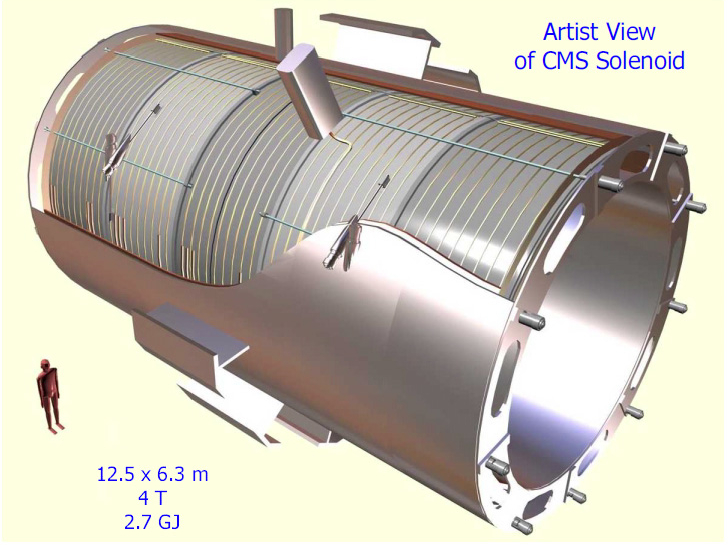
\includegraphics[width=0.6\textwidth]{02_experimental_setup/plots/CERN_CMS_Solenoid_schematic.jpg}
  \caption{The schematic view on the CMS solenoid}
  \label{fig:solenoid}
\end{figure}

%%%%%%%%%%%%%%%%%%%%%%%%%%%%%%%%%%%%%%
\subsection{Tracking Detector}

The inner tracking detector\cite{TrackerTDR, CMSatLHC} (also called tracker) at CMS is the closest component to the beam line and to the collision point having a
length 5.8m and a diameter of 2.5m. It is designed for a precise track and secondary vertex measurement. 
The tracker is positioned inside the solenoid (see Section \ref{ssec:solenoid}) and has a best performance in the areas where the magnetic field
is sizable. This corresponds the central pseudorapidity ranges $|\eta| < 2.5$ thus the most emphasis of the tracker design covers the central
areas. The requirements of high granularity, fast readout and radiation hardness lead to tracker design based entirely on silicon
detectors technologies. The tracking detector consists of \textit{pixel} and \textit{strip} silicon modules
and overall structure is displayed on the Fig.\ref{fig:tracker}.

\begin{itemize}
 \item Pixel detector is located at the closest distance to the proton-proton collision point. It is composed of three co-axial barrel layers (BPIX)
 4.4 cm, 7.3 cm and 10.2 cm far from the beamline and two forward discs (FPIX) on positive and negative z side
 at $\pm$34.5 cm and $\pm$46.5 cm. All together the detector consists of 66 million pixels each of a size $100 \times 150 \mu$m$^2$. The hit
 position resolution of 15-20 $\mu$m was reached\cite{TrackPerf}.
 As shown on the Fig.\ref{fig:tracker} the pixel detector covers the rapidity range $|\eta| < 2.5$.
 
 \item Silicon strip detector composed of ten layers follows right after the pixel detector and reaches the distance of 130 cm far
 from the beamlines. It consists of four inner barrel layers or Tracker Inner Barrel (TIB), two inner endcups each containing 3 discs
 or Tracker Inner Disk (TID), six outer barrel layers or Tracker Outer Barrel (TOB) and two outer Tracker End Cups (TEC).
 Each of the components has a specific design corresponding to it's position and geometry. Overall a silicon tracker consists of 9.3
 million strips.
\end{itemize}

\begin{figure}[t]
  \centering
  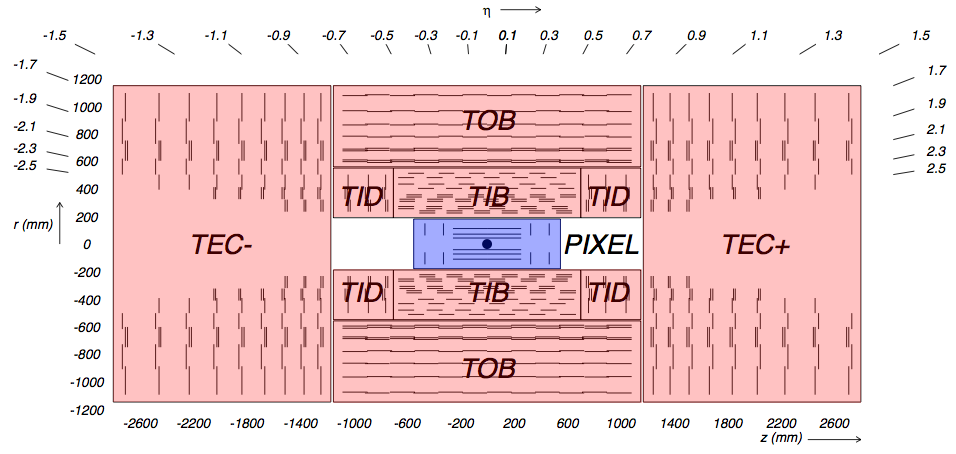
\includegraphics[width=0.8\textwidth]{02_experimental_setup/plots/img_cms_tracker_view.png}
  \caption{CMS tracking detector. The pixel part is marked with blue and the strip part is marked with red.}
  \label{fig:tracker}
\end{figure}

With overall 200 m$^2$ of active silicon area CMS tracking detector became the largest silicon tracker ever built. 

%%%%%%%%%%%%%%%%%%%%%%%%%%%%%%%%%%%%%%
\subsection{Electromagnetic Calorimeter}

The Electromagnetic Calorimeter (ECAL)~\cite{ECALtdr, ECALtdradd, CMSatLHC} is a detector component which comes next after the tracker on the way of particles from
the collision point. The facility is assigned to measure the full electron and photon energies in all the directions. 
A very special lead tungsten (PbWO$_{4}$) scintillating crystal was made to build up the ECAL. The crystalline is heavier then stainless steel but transparent thanks 
to the oxygen touch. Each crystal weights 1.5 kg having a size of a coffee cup.

ECAL is a homogeneous detector made up of a \textit{barrel} part (EB) covering the range of $|\eta| <$ 1.479 and two \textit{endcups} (EE) in the range $(1.479 < |\eta| < 3.0)$
as shown on the Fig.\ref{fig:ecal}. For a high precision low momentum gamma quanta measurement a \textit{Preshower} is installed right before 
the endcups.

\begin{figure}[t]
  \centering
  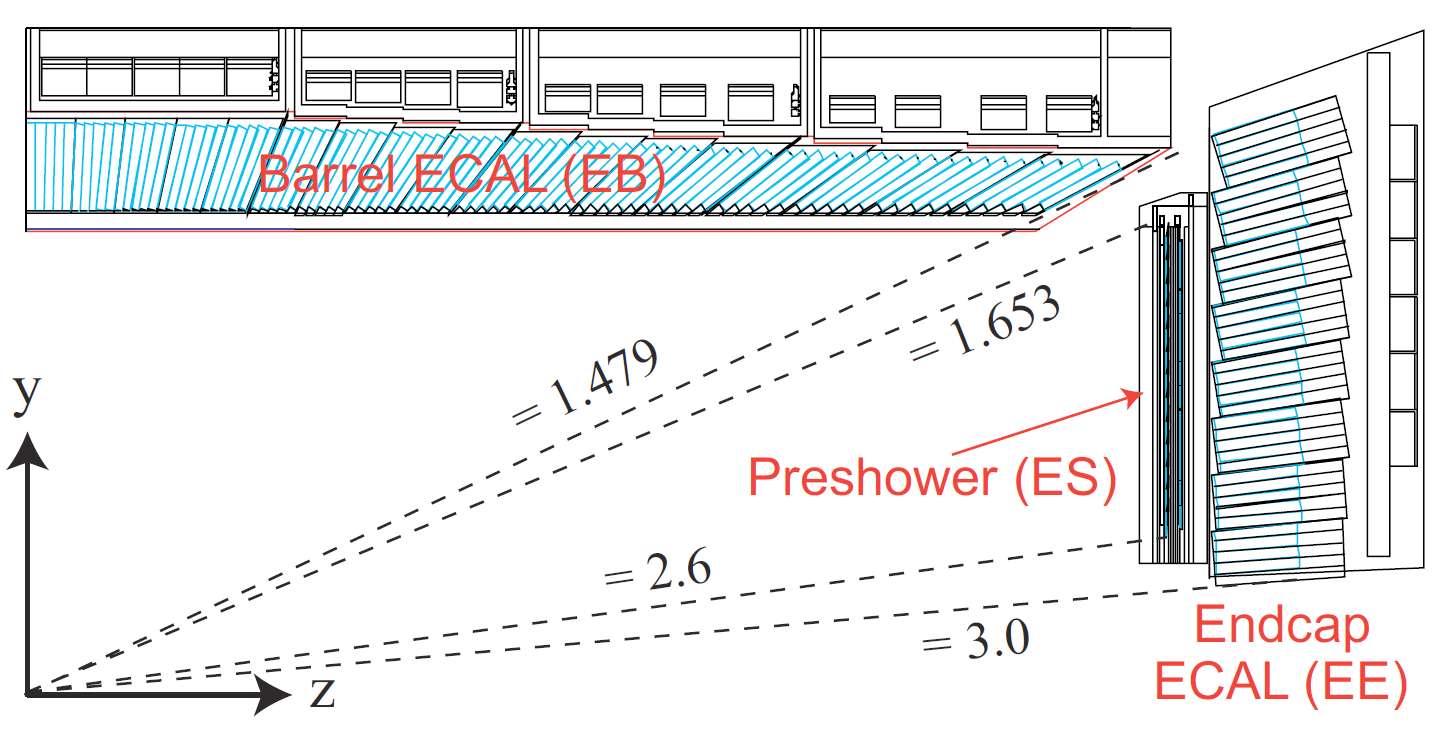
\includegraphics[width=0.8\textwidth]{02_experimental_setup/plots/Figures_Experimental_Apparatus_ECALRapidity.png}
  \caption{CMS electomagnetic calorimeter sketch. Different components and their pseudorapidity ranges are shown.}
  \label{fig:ecal}
\end{figure}

EB of the electromagnetic calorimeter consists of 61200 crystals of lead tungsten joined in modules with 5 crystals in each. It is
cylindrically surrounding the beam pipe starting from the distance of $r = 1.29$m from it. 
The material is dense thus reduces the particle's path allowing a smaller overall size of this detector component. 
Each crystal has a length of 230 mm, corresponding to 25.8$X_{0}$\footnote{A radiation length of electron in PbWO$_{4}$ is 
$X_{0}=0.86$ cm. It corresponds to the distance which an electron should pass in this specific material to reduce it's 
energy by a factor of $\frac{1}{e}$ and to the $\frac{7}{9}$ of the mean free paths for a pair production by a photon.}. 
To avoid the particles traveling through the cracks between the single submodules they are all tilted by 3$^{\circ}$ with 
respect to the direction to the nominal collision point. Lead tungsten scintillation decay time\footnote{Scintillation Decay 
time is the time required for scintillation emission to decrease to $e^{-1}$ of its maximum.} is in order of 25 ns thus it 
emits 80$\%$ of the light signals fast enough to fit into the bunch spacing designed for the LHC. A special avalanche 
photomultiplier designed to work under the high magnetic fields is glued on the back side of each crystal to detect the scintillated light\cite{APDVPT}.

A Preshower forms a 20 cm thick disc which contains two layers of lead to form the showering each followed by a layer of silicon strips to
detect the particles from the shower. A much finer granularity of the silicon strips (2 mm wide each) compared to the 
crystals in EB and EE allow a more accurate particle distinction. An additional cooling to -10$^{\circ}$C -- -15$^{\circ}$C 
of the silicon detectors has to be provided.

EE consists of two endcups each being composed of 7324 lead tungsten crystals placed at $z = \pm 3.154$m. As for the EB the modules
at EE are slightly tilted but each crystal is a bit shorter compared to the barrel layer (24.7$X_{0}$). Vacuum phototriodes\cite{APDVPT} were
glued to the back side of the scintillating planes.

The enegry resolution $\sigma(E)$ of the ECAL detector is given as\cite{CMSatLHC}:

\begin{equation}\label{eq:resECAL}
  (\frac{\sigma}{E})^{2} = (\frac{S}{\sqrt{E}})^{2} + (\frac{N}{E})^{2} + C^{2},
\end{equation} 

where $S$ is a stochastic term due to different measurement fluctuations, $N$ -- a noise term due to electronics and pile up noise
and $C$ -- a constant term due to systematic imperfections and from temperature instabilities. 
The ECAL energy resolution was primary determined on the test beam using 
electrons in the energy range from 20 GeV to 240 GeV\cite{ECALres2007} and taking (\ref{eq:resECAL}) to account the result was the
following:

\begin{equation}\label{eq:resECAL}
  (\frac{\sigma}{E})^{2} = (\frac{2.8\%}{\sqrt{E}})^{2} + (\frac{12\%}{E})^{2} + (0.3\%)^{2}.
\end{equation}

After the measurement of the ECAL characteristics with the proton-proton collisions with the center-of-mass energy $\sqrt{s} = $7 TeV
at the LHC in 2010 and 2011 it was found that for the 60 GeV electrons the energy resolution varies from 1.1$\%$ in barrel to 5$\%$ in 
forward regions\cite{ECALres2013}.

%%%%%%%%%%%%%%%%%%%%%%%%%%%%%%%%%%%%%%
\subsection{Hadron Calorimeter}

The Hadron Calorimeter (HCAL)\cite{CMSatLHC} at CMS follows the ECAL and aims to capture until the full stop all the particles which entered it, 
except for the muons. As it assumed that electrons are absorbed in the ECAL, HCAL is designed to measure the full energy of hadrons. 
Due to the hermiticity, the detector should identify all the hadron decay products. Thus any energy imbalance would point to the
existance of non-interacting neutral particles as neutrinos.

One of the main challenges of the hadronic calorimeter design was to fit it inside the compact solenoid (see sec.\ref{ssec:solenoid}).
The solution was to put one of the parts of the detector component outside the magnet coil. Thus HCAL consists of the barrel (HB), 
outer barrel (HO), endcup (HE) and forward (HF) parts. A schematic sketch of the hadron calotimeter is presented on the Fig.\ref{fig:hcal}.

\begin{figure}[t]
  \centering
  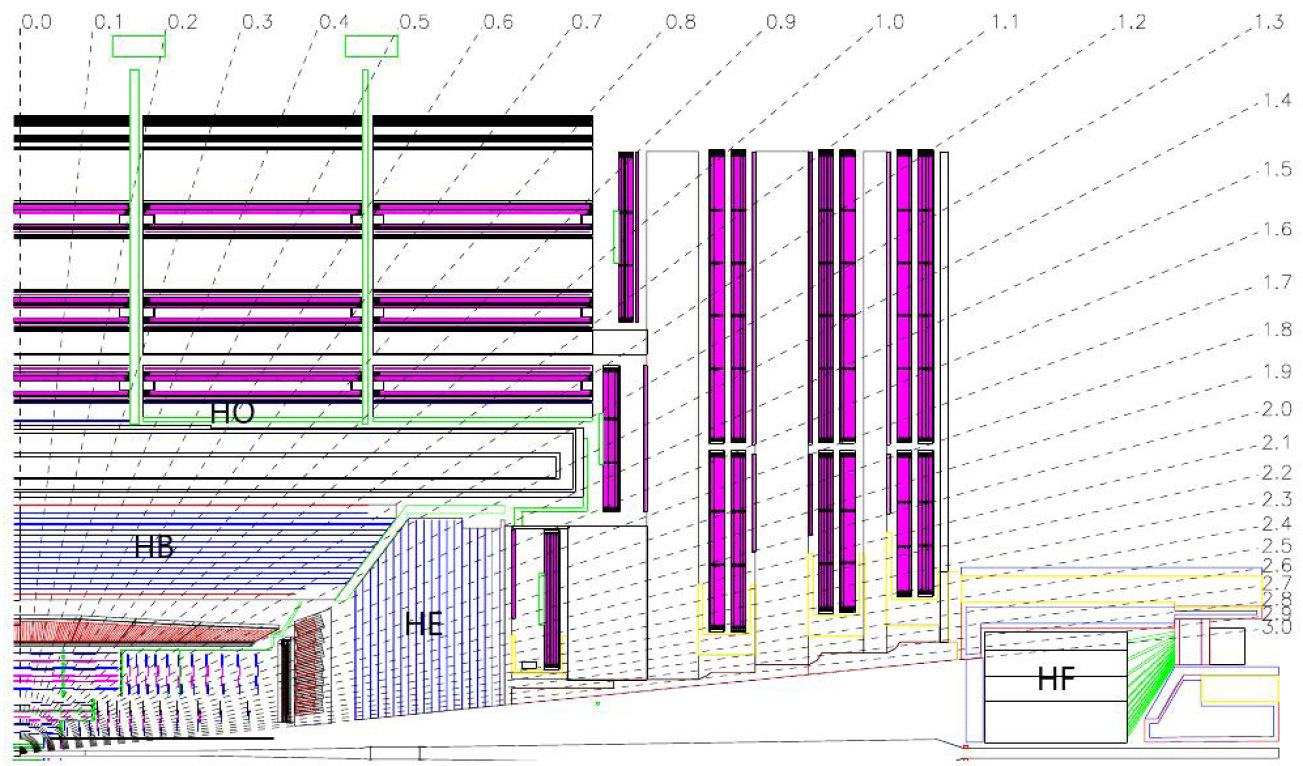
\includegraphics[width=0.6\textwidth]{02_experimental_setup/plots/Figures_Experimental_Apparatus_HCAL.png}
  \caption{CMS hadron calorimeter sketch. Different components and their pseudorapidity ranges are shown.}
  \label{fig:hcal}
\end{figure}

The HB and HE are the sampling calorimeters composed of brass and stainless steel plates (some of them made of Russian Navy brass 
shell casements in World War II) interleaved with scintillators. HB covers the pseudorapidity range of $|\eta| < $1.3. It contains 14 brass and
2 stainless steel absorbers, each from 50.4 mm to 56.6 mm thick. The HE covers more forward region in pseudorapidity -- 1.6$ < |\eta| < $3.0. It is composed
of 18 layers of 79 mm thick brass plates. The scintillator plastic tiles are located after each absorber layer. The gaps between tiles are covered 
with reflective paint to keep the light emitted inside one scintillator plate doesn't travel outside as this light gives the energy estimate. Optic fibers fitted into
specially cut grooves on top of scintillating tiles collect light signals and pass them to the readout boxes with hybrid photodiodes. The signals
collected from successive tiles, one behind the other, are optically added and form so called ``towers``. The towers are indicating 
the particle path in the calorimeter.

HB and HE material thickness provides only 5.82$\lambda_{I}$\footnote{$\lambda_{I}$ is a \textit{nuclear interaction length}, or the average 
length the particle has to travel inside the material before undergoing an inelastic nuclear interaction} in central region to 10.6$\lambda_{I}$ in more forward once. The 
ECAL material overall is equal to 1.1$\lambda_{I}$. This is not enough to stop all the hadron showers\footnote{To fully contain a 1 TeV hadronic jet a thickness of
roughly 11$\lambda_{I}$.} so the additional outer calorimeter HO
was placed outside the solenoid. Using the solenoid and yoke material itself, adding also some own absorber plates, HO provides 11.6$\lambda_{I}$ in the
most central regions.

The forward calorimeter part HF starts from the $z = \pm$11.6 m distance covering the pseudorapidity range of 3.0$ < |\eta| < $5.2. It has a cylindrical shape
with the inner radius $r = $12.5 cm and outer radius $r = $130.0 cm. The overall length of HF is 165 cm. It consists of absorbing steel grooved plates and
quartz light emitting tubes placed in these groves parallel to the beam pipe. As the HF faces not only hadronic but also the electromagnetic radiation
it has to be sensitive to both. Thus half of the quartz tubes spread over the whole length of the HF (165 cm) and the other half starts only at 22 cm 
from the front side of the HF. The long and the short quartz fibers have different readouts. Electromagnetic showers would start very early  not reaching the 
short quartz tubes.

%%%%%%%%%%%%%%%%%%%%%%%%%%%%%%%%%%%%%%
\subsection{Muon Detector}

The Muon Detector\cite{CMSatLHC} together with the solenoid is a name giving part of the CMS experimental setup. As muons pass through calorimeter materials
without significant losses\cite{MuonStop}, muon detection systems can be placed on the outer layers of the whole CMS facility. A very precize measurement of muons 
is possible also combining with a tracking detector. The unique signature of a muon in the event can be used for triggering. Muons appear in the processes
of most physical interest at CMS, like Higgs or heavy resonances decays.

Muon system stations are located outside the solenoid and in-between the return yoke plates. A muon track is fitted to the hits in each station 
and interpolated to the tracker. That is why muon system and the central tracking detector are aligned within one sixth of a millimeter.

The muon detector consists of 1400 gaseous chambers of three types: 250 Drift Tubes (DT), located in barrel region of $|\eta| < $1.2, 540 Cathode Strip Chambers
(CSC) as endcups covering the pseudorapidity of 0.9$ < |\eta| < $2.4 and 610 Resistive Plate Chambers (RPC) placed in both, barrel and endcup regions, and covering
the range $|\eta| < $1.6. A schematic view of the muon detecting system with its components is presented on Fig.\ref{fig:muond}.

\begin{figure}[t]
  \centering
  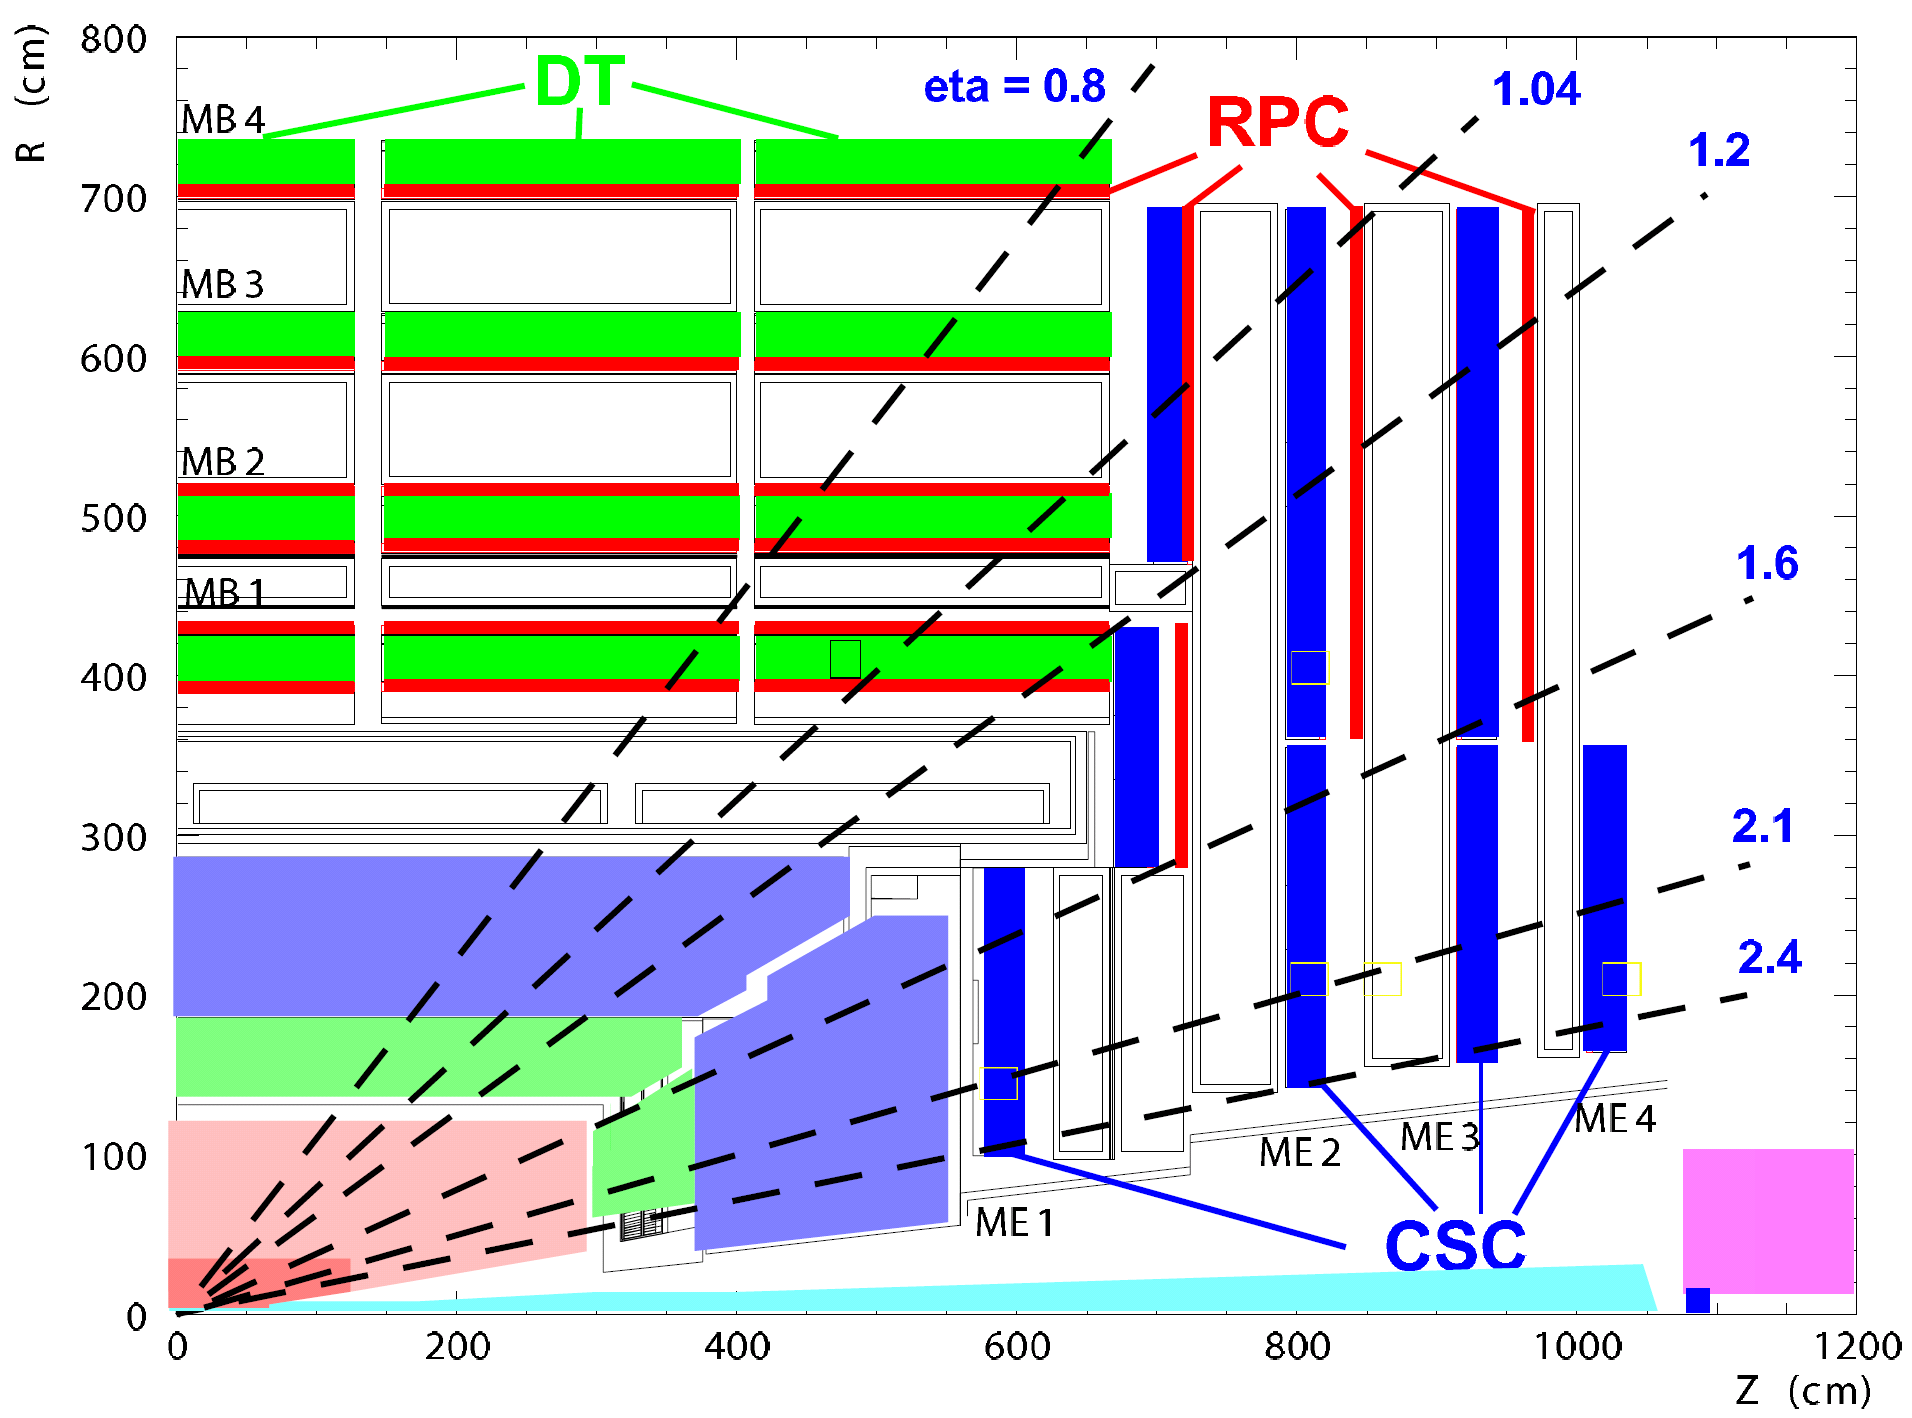
\includegraphics[width=0.6\textwidth]{02_experimental_setup/plots/Figures_Experimental_Apparatus_MuonDetector.png}
  \caption{CMS hadron calorimeter sketch. Different components and their pseudorapidity ranges are shown.}
  \label{fig:muond}
\end{figure}

The DT measures muon position with a help of the system of 4 cm wide gas tubes filled with 15$\%$ of Argon and 85$\%$ of carbon dioxide.
Each tube contains a stretched positively charged wire inside to collect the charge from the gas ionized by muons.

% \subsection{Trigger system}
% \subsection{Data quality monitoring}
% 
% \section{Upgrade for RunII}
% \subsection{CMS Pixel Tracker Upgrade}